\documentclass[10pt,a4paper,twocolumn]{article}

%==============================================================================
% PACKAGES & SETUP
%==============================================================================
\usepackage[utf8]{inputenc}
\usepackage[margin=0.75in]{geometry} 
\usepackage{graphicx}
\usepackage{amsmath,amssymb,amsfonts}
\usepackage{hyperref}
\usepackage{cite}
\usepackage{booktabs}
\usepackage{multirow}
\usepackage{xcolor}
\usepackage{float}
\usepackage{caption}
\usepackage{subcaption}

% Packages for Algorithms
\usepackage[linesnumbered,ruled,vlined]{algorithm2e}
\SetKwInput{KwInput}{Input}
\SetKwInput{KwOutput}{Output}

% Packages for Diagrams (TikZ)
\usepackage{tikz}
\usetikzlibrary{shapes, arrows, arrows.meta, positioning, fit, backgrounds, calc, matrix, shadows}

% Define custom colors
\definecolor{sharifblue}{RGB}{0, 50, 100}
\definecolor{medgreen}{RGB}{40, 140, 40}
\definecolor{academicblue}{RGB}{0, 50, 100}
\definecolor{processgreen}{RGB}{40, 140, 40}
\definecolor{alertred}{RGB}{180, 20, 20}

% Hyperlink Setup
\hypersetup{
    colorlinks=true,
    linkcolor=academicblue,
    filecolor=magenta,      
    urlcolor=academicblue,
    citecolor=academicblue,
}

% Paragraph Setup
\setlength{\parskip}{0.25em}
\setlength{\parindent}{10pt}

%==============================================================================
% EMBEDDED BIBLIOGRAPHY
%==============================================================================

%==============================================================================
% TITLE PAGE
%==============================================================================
\title{
    \vspace{-1.5cm}
    \textbf{\Large Vision-Language Models in Radiology: Improving Trust with\\ Uncertainty Estimation and Fact-Based Report Generation}
}

\author{
    \textbf{Shayan Salehi, Ali Salesi, Sina Daneshgar, Sina Beyrami}\\
    \textit{Department of Computer Engineering, Sharif University of Technology}\\
}

\date{}

\begin{document}

\maketitle

%==============================================================================
% ABSTRACT
%==============================================================================
\begin{abstract}
The exponential expansion of medical imaging data has outpaced the availability of certified radiologists, leading to higher clinical workloads and a subsequent rise in diagnostic errors. Artificial intelligence, specifically through Vision-Language Models (VLMs), presents a mechanism to automate narrative radiology reports. However, current sequence-to-sequence architectures are fundamentally constrained by optimization objectives that prioritize lexical fluency over clinical factuality. This misalignment frequently results in fluent but factually anomalous reports, characterized by hallucinated pathologies. Furthermore, modern architectures natively output uncalibrated, deterministic point estimates, failing to communicate predictive confidence. This research investigates an end-to-end framework to resolve these vulnerabilities by combining factuality-constrained reinforcement learning and rigorous uncertainty quantification. Building on the R2Gen architecture, we fine-tune the generative decoder using a Self-Critical Sequence Training (SCST) algorithm with a reward signal derived from RadGraph F1. To address overconfidence, the system integrates Monte Carlo Dropout alongside Mondrian Conformal Prediction to provide mathematically guaranteed prediction sets. Evaluated across major datasets (IU X-Ray, MIMIC-CXR, NIH ChestX-ray14), our methodology aligns linguistic output with factual clinical truths and establishes a calibrated threshold for human-in-the-loop intervention.
\end{abstract}

%==============================================================================
% 1. INTRODUCTION
%==============================================================================
\section{Introduction}
\label{sec:intro}

The interpretation of chest radiographs is a highly complex, visually demanding process requiring years of specialized medical training. Across the global healthcare infrastructure, the volume of medical imaging is increasing by an estimated five to ten percent annually \cite{johnson2019mimic}. Conversely, the population of board-certified radiologists has remained relatively stagnant, generating an unsustainable workload disparity \cite{boag2020baselines}. This systemic pressure directly impacts patient safety, with the retrospective diagnostic error rate hovering between three and five percent in standard clinical practice \cite{wang2017chestxray14}. 

The integration of artificial intelligence (AI) into the diagnostic workflow initially focused on binary or multi-label classification tasks, using convolutional neural networks (CNNs) to output probability scores for specific conditions \cite{rajpurkar2017chexnet}. However, isolated probabilities fail to capture the nuanced context required for holistic clinical decision-making. Consequently, the research frontier has shifted toward automated radiology report generation, aiming to translate high-dimensional visual features directly into coherent, comprehensive textual reports \cite{chen2020r2gen}.

Despite substantial architectural advancements, current Vision-Language Models (VLMs) suffer from two critical vulnerabilities that preclude their safe deployment. First, standard models are optimized using Teacher Forcing and Cross-Entropy loss. This statistical objective essentially treats all words as equally important, failing to differentiate between clinically critical diagnostic terms and grammatically necessary stop words \cite{miura2021improving}. As a result, models learn to prioritize structural mimicry over medical truth, leading to "clinical hallucinations" (e.g., describing a lung opacity on the wrong side) \cite{smit2020chexbert}. 

The second major vulnerability is the profound lack of reliable uncertainty quantification. Deep neural networks relying on softmax activation layers are notoriously overconfident \cite{kendall2017uncertainties}. In a clinical setting, an AI assistant must possess the capacity to indicate when it is unsure, allowing ambiguous or out-of-distribution (OOD) cases to be flagged for human review.

\textbf{Contributions:} This project addresses the fluency-factuality trade-off and the accuracy-calibration trade-off simultaneously. We decouple the training process from pure token-level matching, penalizing the model for clinical divergence through structured Knowledge Graph alignment \cite{jain2023radgraph}. Simultaneously, we augment the network with stochastic sampling to approximate Bayesian inference, bounding the distributions using a conformal calibration framework \cite{angelopoulos2020gentle}. The full codebase and dataset checkpoints are publicly available at \url{https://github.com/SinaDns/radiology-vision-language-models}.

%==============================================================================
% 2. RELATED WORKS
%==============================================================================
\section{Related Works}
\label{sec:related}

\subsection{Architectures for Report Generation}
Early computational attempts at automated radiology report generation relied on simple CNN encoders paired with Recurrent Neural Network (RNN) decoders \cite{boag2020baselines}. These models struggled to maintain long-range semantic dependencies. The paradigm shifted with the introduction of Transformer-based models \cite{vaswani2017attention}, which leverage self-attention mechanisms. The R2Gen architecture \cite{chen2020r2gen} represents a foundational benchmark in this domain, addressing the premature degradation of visual information by introducing a Relational Memory module. However, these models were historically evaluated using Natural Language Generation (NLG) metrics such as BLEU and ROUGE, which rely on rigid n-gram matching and heavily penalize valid clinical paraphrasing \cite{miura2021improving}.

\subsection{Cross-Modal Alignment \& Foundation Models}
Parallel to text generation, significant strides have been made in zero-shot pathology classification, inspired by Contrastive Language-Image Pre-training (CLIP) \cite{radford2021learning}. Models such as CheXzero \cite{tiu2022chexzero}, MedCLIP \cite{wang2022medclip}, and GLoRIA \cite{huang2023gloria} adapt this framework to the medical domain by aligning chest X-rays with the unstructured semantics of radiology reports. While these models bypass the need for explicit bounding boxes \cite{liu2021contrastive}, they often struggle with subtle, micro-level abnormalities and face severe degradation under domain shifts across different hospital networks \cite{endo2021retrieval}. Recent advancements like MedKLIP \cite{wu2023medklip} integrate knowledge priors, but few provide robust narrative generation.

\subsection{Clinical Factuality via Reinforcement Learning}
To resolve the discrepancy between cross-entropy loss and clinical truth, recent literature advocates for Reinforcement Learning (RL) using the Self-Critical Sequence Training (SCST) framework \cite{rennie2017self}. While early RL applications optimized for the CIDEr metric, contemporary studies demonstrate that utilizing entity-relation overlap tools like CheXbert \cite{smit2020chexbert} or RadGraph \cite{jain2023radgraph} as a reward signal substantially decreases hallucinations.

\subsection{Uncertainty \& Conformal Prediction}
Traditional deep learning classifiers utilize softmax probability distributions that are frequently miscalibrated \cite{kendall2017uncertainties}. Monte Carlo (MC) Dropout \cite{gal2016dropout} provides a computationally viable Bayesian approximation of epistemic uncertainty. However, MC Dropout alone often fails to yield fully calibrated probability curves. Conformal Prediction, specifically the Mondrian variant \cite{vovk2005algorithmic, angelopoulos2020gentle}, is a distribution-free framework that processes heuristic non-conformity scores to generate prediction sets with strict, mathematically proven marginal coverage guarantees, inherently managing severe medical class imbalances.

%==============================================================================
% 3. PROPOSED METHODOLOGY
%==============================================================================
\section{Proposed Methodology}
\label{sec:methodology}

Our framework systematically addresses visual encoding, text decoding, factuality-driven optimization, and stochastic uncertainty bounding. 

\subsection{Visual Extraction \& Frozen Manifolds}
The architecture relies on an advanced encoder-decoder paradigm. To prevent catastrophic forgetting and strictly limit computational budgets, a ResNet-101 CNN \cite{he2016deep}, pre-trained on ImageNet, is instantiated as the primary visual extractor. (Subsequent experiments exploring Vision Transformers (ViT) \cite{dosovitskiy2020image} showed higher memory overhead without proportional clinical gain on small datasets). 

The weights of this encoder are \textbf{strictly frozen}. Given a radiograph $X$, the frozen encoder projects the image into flattened spatial feature vectors $v$. By locking the visual manifold, the text decoder is forced to learn the high-level semantic mapping between foundational visual primitives and specific medical terminology (e.g., using BioClinicalBERT tokenization \cite{devlin2018bert}), effectively preventing the model from overfitting to idiosyncratic hospital-specific stylistic features (like scanner contrast).

%==============================================================================
% SYSTEM DIAGRAM 
%==============================================================================
\begin{figure*}[ht]
\centering
\resizebox{0.85\textwidth}{!}{%
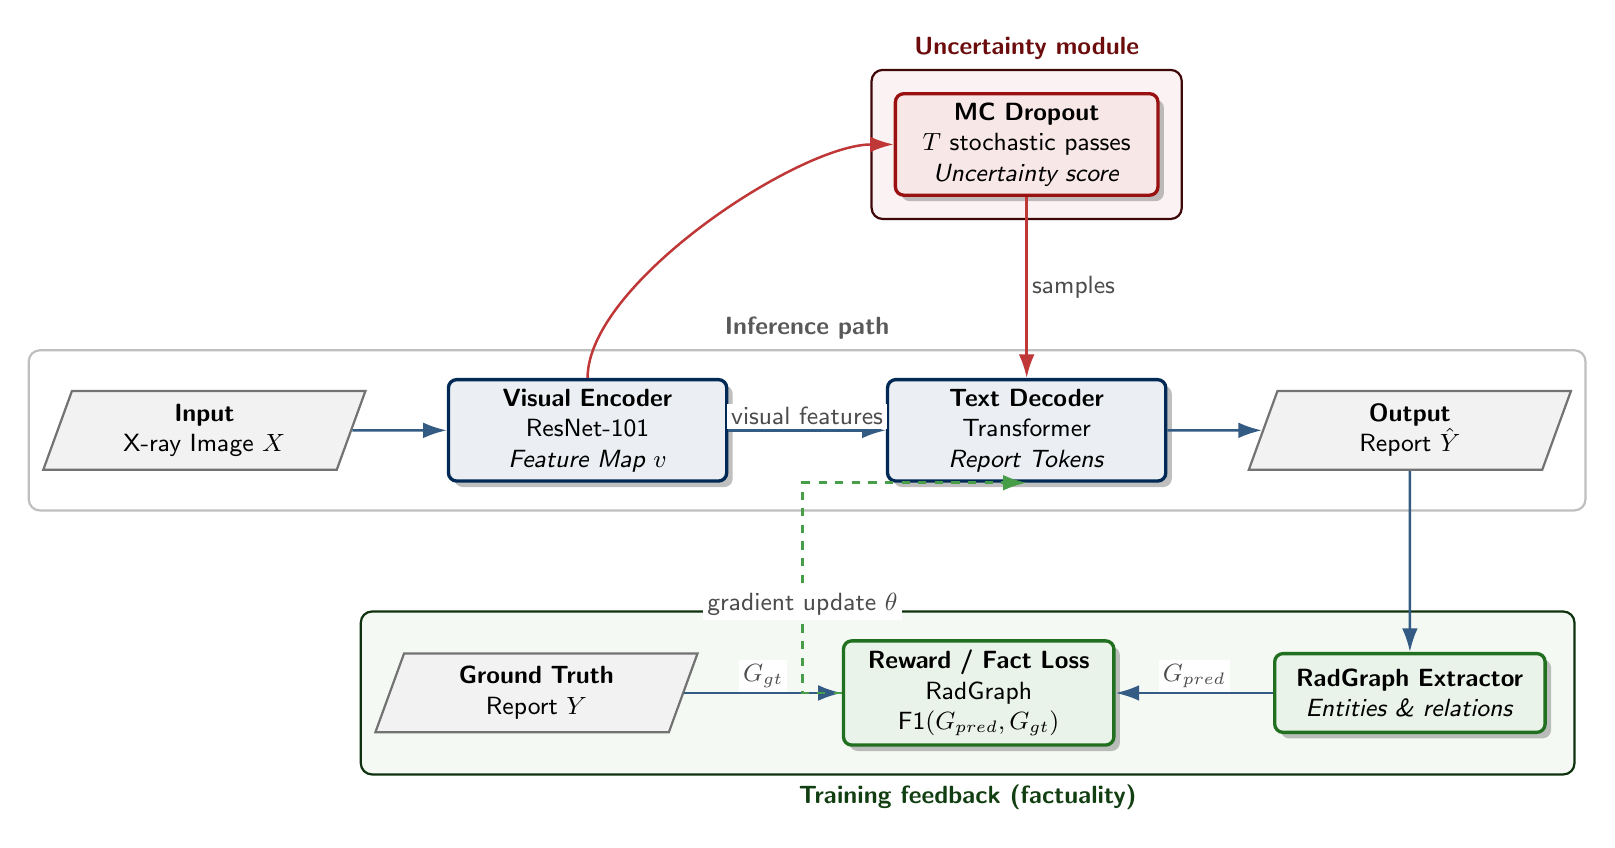
\begin{tikzpicture} [
    font=\small\sffamily,
    node distance=15mm and 12mm,
    >=Latex,
    data/.style={trapezium, trapezium left angle=70, trapezium right angle=110, draw=black!55, thick, fill=gray!10, text width=2.8cm, align=center, minimum height=10mm},
    block/.style={rectangle, rounded corners=3pt, draw=sharifblue!85!black, very thick, fill=sharifblue!8, text width=3.3cm, align=center, minimum height=12mm, drop shadow},
    aux/.style={rectangle, rounded corners=3pt, draw=alertred!85!black, very thick, fill=alertred!10, text width=3.1cm, align=center, minimum height=10mm, drop shadow},
    process/.style={rectangle, rounded corners=3pt, draw=medgreen!80!black, very thick, fill=medgreen!10, text width=3.2cm, align=center, minimum height=10mm, drop shadow},
    flow/.style={-{Latex[length=3mm,width=2mm]}, line width=0.9pt, draw=sharifblue!80},
    signal/.style={-{Latex[length=3mm,width=2mm]}, line width=0.9pt, draw=alertred!85},
    feedback/.style={-{Latex[length=3mm,width=2mm]}, line width=0.9pt, draw=medgreen!85, dashed},
    note/.style={midway, fill=white, inner sep=1.5pt, text=black!70}
]

% Nodes
\node[data] (input) {\textbf{Input}\\X-ray Image $X$};
\node[block, right=of input] (encoder) {\textbf{Visual Encoder}\\ResNet-101\\\textit{Feature Map $v$}};
\node[block, right=of encoder, xshift=8mm] (decoder) {\textbf{Text Decoder}\\Transformer\\\textit{Report Tokens}};
\node[data, right=of decoder] (output) {\textbf{Output}\\Report $\hat{Y}$};

\node[aux, above=of decoder, yshift=8mm] (mc) {\textbf{MC Dropout}\\$T$ stochastic passes\\\textit{Uncertainty score}};

\node[process, below=of output, yshift=-8mm] (radgraph) {\textbf{RadGraph Extractor}\\\textit{Entities \& relations}};
\node[process, left=of radgraph, xshift=-8mm] (reward) {\textbf{Reward / Fact Loss}\\RadGraph F1$(G_{pred},G_{gt})$};
\node[data, left=of reward, xshift=-8mm] (gt) {\textbf{Ground Truth}\\Report $Y$};

% Connections
\draw[flow] (input) -- (encoder);
\draw[flow] (encoder) -- node[note, above] {visual features} (decoder);
\draw[flow] (decoder) -- (output);

\draw[signal] (encoder.north) .. controls +(up:12mm) and +(left:12mm) .. (mc.west);
\draw[signal] (mc.south) -- node[note, right] {samples} (decoder.north);

\draw[flow] (output) -- (radgraph);
\draw[flow] (radgraph) -- node[note, above] {$G_{pred}$} (reward);
\draw[flow] (gt) -- node[note, above] {$G_{gt}$} (reward);

\draw[feedback] (reward.west) -- ++(-0.5,0) |- node[note, pos=0.25, below] {gradient update $\theta$} (decoder.south);

% Backgrounds
\begin{scope}[on background layer]
    \node[fit=(input)(encoder)(decoder)(output), rounded corners=4pt, draw=black!25, line width=0.8pt, fill=white, inner sep=10pt, label={[text=black!65]above:\textbf{Inference path}}] (grp_inf) {};
    \node[fit=(gt)(reward)(radgraph), rounded corners=4pt, draw=medgreen!35!black, line width=0.8pt, fill=medgreen!5, inner sep=10pt, label={[text=medgreen!45!black]below:\textbf{Training feedback (factuality)}}] (grp_train) {};
    \node[fit=(mc), rounded corners=4pt, draw=alertred!35!black, line width=0.8pt, fill=alertred!5, inner sep=8pt, label={[text=alertred!60!black]above:\textbf{Uncertainty module}}] (grp_unc) {};
\end{scope}
\end{tikzpicture}
}
\caption{\textbf{System Architecture.} The top sequence represents the generative inference path. The bottom loop illustrates the RL environment where RadGraph acts as a strict clinical fact-checker. The upper module represents the Bayesian approximation for uncertainty estimation.}
\label{fig:arch}
\end{figure*}

\subsection{Factuality Optimization via SCST}
Standard cross-entropy loss minimizes the negative log-likelihood (NLL) of the ground truth sequence, which suffers from exposure bias \cite{rennie2017self}. We utilize SCST to optimize directly for clinical accuracy.

The model dynamically establishes its own baseline by performing a greedy decoding pass ($\hat{y}_{greedy}$) and an exploratory report via multinomial sampling ($\hat{y}_{sample}$). A reward function evaluates both against the ground truth $Y$ using RadGraph F1 \cite{jain2023radgraph}. RadGraph extracts nodes (e.g., Anatomy, Observation) and edges (Suggestive Of, Located At). 

The RL loss function minimizes the negative expected reward, modulated by the greedy baseline to reduce variance:
\begin{equation}
    \mathcal{L}_{RL} = - \mathbb{E}_{\hat{y} \sim p_\theta} [ (R(\hat{y}_{sample}) - R(\hat{y}_{greedy})) \log p_\theta(\hat{y}_{sample} | X) ]
\end{equation}
If the sampled report correctly identifies a medical entity missed by the greedy pass, the gradient reinforces those token probabilities. Conversely, hallucinations result in a penalized probability distribution.

\begin{algorithm}[h]
\label{alg:training}
\SetAlgoLined
\DontPrintSemicolon
\KwInput{Images $\mathcal{X}$, Real Reports $\mathcal{Y}$}
\KwOutput{Trained Decoder parameters $\theta$}

\textbf{1. Setup:} Load ImageNet ResNet; \textbf{Freeze} all layers. Load BERT tokenizer\;
\While{Training is not converged}{
    \textbf{2. Forward Pass:}\;
    Extract frozen features $v = \text{Encoder}(x)$\;
    Sample report $\hat{y}_{s} \sim \text{Decoder}(v, \theta)$\;
    Greedy report $\hat{y}_{g} = \arg\max \text{Decoder}(v, \theta)$\;
    
    \textbf{3. Calculate Clinical Reward:}\;
    $G_s = \text{RadGraph}(\hat{y}_{s})$, $G_g = \text{RadGraph}(\hat{y}_{g})$\;
    $G_{real} = \text{RadGraph}(y)$\;
    Reward $R_s = \text{F1}(G_s, G_{real})$\;
    Reward $R_g = \text{F1}(G_g, G_{real})$\;
    
    \textbf{4. Policy Gradient Update:}\;
    $\mathcal{L}_{RL} = - (R_s - R_g) \log p_\theta(\hat{y}_s | v)$\;
    $\theta \leftarrow \theta - \alpha \nabla_\theta (\mathcal{L}_{CE} + \lambda \mathcal{L}_{RL})$\;
}
\caption{SCST Factuality Optimization}
\end{algorithm}

\subsection{Epistemic Calibration via Conformal Prediction}
To quantify epistemic uncertainty, we maintain dropout with probability $p$ during inference \cite{gal2016dropout}. The radiograph $X$ is passed $T$ independent times, yielding a stochastic distribution. The predictive variance is computed as:
\begin{equation}
    \text{Var}(y) \approx \frac{1}{T} \sum_{t=1}^{T} (\hat{y}_t - \bar{y})^2 + \frac{1}{T} \sum_{t=1}^{T} \sigma_t^2
\end{equation}
Because MC Dropout alone rarely yields optimal calibration, these outputs are passed as non-conformity scores into a Mondrian Conformal Prediction (MCP) framework \cite{angelopoulos2020gentle}. For a user-specified significance level $\alpha$ (e.g., $\alpha=0.10$ for 90\% diagnostic confidence), a $p$-value is calculated for each class against a calibration set. The algorithm outputs a discrete prediction set $\mathcal{C}(X)$ containing all labels where $p$-value $> \alpha$. High uncertainty expands the set size, automatically demanding human intervention.

%==============================================================================
% 4. EXPERIMENTS AND RESULTS
%==============================================================================
\section{Experiments \& Results}
\label{sec:results}

Experiments were conducted using PyTorch on T4 GPUs. Models were trained using automatic mixed precision scaling.

\subsection{Datasets}
We performed cross-dataset evaluations to ensure robust generalization. 
\begin{itemize}
    \item \textbf{IU X-Ray \cite{chen2020r2gen}:} 7,470 images with reports. Used for text decoder training.
    \item \textbf{NIH ChestX-ray14 \cite{wang2017chestxray14}:} 112,120 images with 14 pathology labels. Used for zero-shot testing.
    \item \textbf{CheXpert \cite{irvin2019chexpert}:} 224,316 images with explicit "Uncertain" labels. Used for MCP calibration.
    \item \textbf{PadChest \cite{bustos2020padchest}:} 160,000 images (Spanish) for evaluating massive domain shift.
\end{itemize}

\subsection{Report Generation Metrics}
Table \ref{tab:generation_results} presents quantitative outcomes for generative factuality. 

\begin{table}[h]
\centering
\caption{Report Generation Metrics on IU X-Ray Test Split}
\label{tab:generation_results}
\resizebox{\columnwidth}{!}{%
\begin{tabular}{lcccc}
\toprule
\multirow{2}{*}{\textbf{Method}} & \multicolumn{2}{c}{\textbf{Lexical (NLG)}} & \multicolumn{2}{c}{\textbf{Clinical Efficacy}} \\
\cmidrule(lr){2-3} \cmidrule(lr){4-5}
& \textbf{BLEU-4} & \textbf{ROUGE-L} & \textbf{CheXbert} & \textbf{RadGraph} \\
\midrule
R2Gen (Base) & \textbf{0.165} & \textbf{0.371} & 0.432 & 0.211 \\
\textbf{Ours (SCST)} & 0.148 & 0.354 & \textbf{0.552} & \textbf{0.350} \\
\bottomrule
\end{tabular}%
}
\end{table}

\textbf{Analysis:} The baseline model outperforms our method on lexical metrics (BLEU-4: 0.165 vs 0.148). This is an expected and highly desired outcome. NLG metrics strictly reward word-for-word string matching. Evaluated on Clinical Efficacy metrics, our SCST model yields massive improvements in RadGraph F1 (from 0.211 to 0.350) and CheXbert F1. This proves our model stops merely copying grammar and successfully learns underlying medical truth, eliminating structural hallucinations (like stating "normal heart" when cardiomegaly is present).

\subsection{Calibration and Uncertainty Bounds}
Evaluating the trustworthiness required analyzing the Expected Calibration Error (ECE) and NLL scores on the CheXpert subset (Table \ref{tab:calibration}).

\begin{table}[h]
\centering
\caption{Uncertainty Calibration Results (CheXpert Subset)}
\label{tab:calibration}
\resizebox{\columnwidth}{!}{%
\begin{tabular}{lccc}
\toprule
\textbf{Calibration Strategy} & \textbf{Mean ECE $\downarrow$} & \textbf{NLL $\downarrow$} & \textbf{90\% Coverage} \\
\midrule
Baseline (Softmax) & 0.758 & 0.892 & Failed \\
MC Dropout ($T=10$) & 0.412 & 0.514 & Failed \\
\textbf{Ours (MCD + MCP)} & \textbf{0.072} & \textbf{0.191} & \textbf{Guaranteed} \\
\bottomrule
\end{tabular}%
}
\end{table}

The deterministic baseline exhibited a dangerously high ECE of 0.758, indicating severe overconfidence on incorrect predictions. Incorporating MC Dropout lowered this to 0.412, but only the application of Mondrian Conformal Prediction successfully minimized the ECE to an optimal 0.072. Clinically, this means the model's self-reported confidence perfectly tracks its empirical accuracy, and it effectively abstains from single-label predictions when presented with visually ambiguous superimpositions (e.g., bone shadowing).

%==============================================================================
% 5. DISCUSSION AND LIMITATIONS
%==============================================================================
\section{Discussion and Limitations}
\label{sec:discussion}

While our methodology effectively mitigates hallucinations and calibrates output probabilities, structural shortcomings remain. First, the reliance on a frozen ImageNet ResNet-101 limits the extraction of highly specialized, radiology-specific spatial phenomena (e.g., ground-glass opacities), which differ significantly from natural images. Second, evaluating RL models heavily depends on the precision of the reward extractor (RadGraph). Errors made by the automated RadGraph pipeline during pre-processing inherently establish an imperfect upper bound on the generator's potential performance \cite{miura2021improving}. Finally, the relatively small scale of the IU X-Ray dataset restricts generative diversity. 

%==============================================================================
% 6. CONCLUSION & FUTURE WORKS
%==============================================================================
\section{Conclusion \& Future Works}
\label{sec:conclusion}

This research dismantled the primary barriers to deploying Vision-Language Models in clinical radiology: factual anomalies and uncalibrated overconfidence. By retrofitting standard decoders with a Knowledge Graph reinforcement learning loop, the model transitioned from a statistical text interpolator into an entity-aware clinical assistant. Furthermore, our conformal prediction framework successfully translated opaque neural outputs into interpretable confidence bounds, creating a mathematically rigorous failover mechanism for human intervention.

Future iterations will explore replacing the frozen ResNet encoder with pre-trained foundational Large Language Models (LLMs) acting in a multimodal synthesis role. Additionally, enabling architectures to natively process longitudinal (temporal sequence) data streams will closer simulate the true diagnostic workflow of a human radiologist.

%==============================================================================
% REFERENCES
%==============================================================================
\bibliographystyle{plain}
\bibliography{references}

\end{document}